\documentclass[11pt]{article}

\usepackage[margin=1in]{geometry}
\usepackage[utf8]{inputenc}
\usepackage[T1]{fontenc}
\usepackage{amsmath,amssymb}
\usepackage{booktabs}
\usepackage[numbers]{natbib}
\usepackage{hyperref}
\usepackage{enumitem}
\usepackage{caption}
\usepackage{titlesec}
\usepackage{xcolor}
\usepackage{graphicx}

\hypersetup{colorlinks=true,linkcolor=black,citecolor=black,urlcolor=blue!50!black}
\titleformat{\section}{\normalfont\large\bfseries}{\thesection}{0.6em}{}
\titleformat{\subsection}{\normalfont\bfseries}{\thesubsection}{0.6em}{}

\newcommand{\hstar}{H^{*}}

\title{\textbf{False Epistemic Redundancy}\\
\large Do AI Ensembles Share a Blind Spot?}

\author{
Sofia G. Gallego$^{1}$ \and Anya Habana$^{2}$ \\[4pt]
\normalsize $^1$Cosmoventures, Paris, France \quad $^2$University of Edinburgh, Edinburgh, United Kingdom
}
\date{Apart Research Digital Minds Research Sprint, August 2026}

\begin{document}
\maketitle

\begin{abstract}
Multiple AI instances are increasingly consulted the way multiple human
experts would be, with the spread of their opinions sometimes treated as
a proxy for independent judgment. We test this assumption at small scale:
whether differently-prompted copies of one language model, applied to
real, previously investigated cases with a non-obvious established cause,
search their way to that cause or instead share a blind spot inherited
from training. Using three documented cases -- an aviation accident, an
industrial chemical fire, and a newborn's undiagnosed illness -- and two
easier cases as positive controls, we elicited free-text hypotheses from
a language model under a neutral baseline framing and four purpose-built
reasoning personas, with no candidate list and no hint of the answer. The
model recovered the true cause in 0 of 40 hard-case attempts against 40
of 40 control attempts, despite rating each hard-case cause as plausible
once named. Given the complete evidentiary file investigators actually
used, recovery stayed at zero for the aviation case but turned
persona-dependent for the other two, in opposite directions: personas
recovered the industrial cause where baseline did not, and baseline
recovered the medical cause where personas did not. Diversity of wording
and mechanism rose under persona conditioning regardless of this outcome
-- consistent with diversity and correctness being distinct quantities
here, though our sample cannot establish how general that pattern is. The
model's own confidence carried a limited but non-trivial signal for
correctness (AUC 0.70). Taken together, this small-scale test points to a
possible risk worth further study: persona diversity may create an
appearance of independent search without reliably raising its coverage,
whether personas help may depend on a case's answer structure rather than
the personas themselves, and a model's own confidence is not, on this
evidence, a safe substitute for independent expert review. We present
this as an initial, exploratory demonstration rather than a general
result, and outline the additional cases, model families, and fine-tuned
personas needed to test how far it extends.
\end{abstract}

\noindent\textbf{Keywords:} AI safety --- multi-agent systems --- epistemic diversity --- persona conditioning --- common-mode failure --- digital minds

\section{Introduction}

It is becoming common to query several differently-configured instances of
the same AI model and treat their combined output as carrying the weight
of independent judgment -- cross-checking a diagnosis, auditing an
engineering conclusion, or triaging a security incident with a panel of AI
reviewers instead of one. This practice is a bet: that the panel's
individual searches are independent enough for their agreement, or their
collective silence on a possibility, to mean something. This paper puts
that bet to a direct, concrete test: on real problems whose right answer
turned out to be unexpected, does a panel of differently-prompted AI
investigators actually explore its way toward that answer, or does the
whole panel quietly overlook the same possibility together?

A substantial literature shows that instruction-tuned language models
produce markedly less output diversity than their apparent flexibility
suggests \citep{kirk2023,yun2025}, and that this homogeneity propagates
into human-AI co-creation \citep{anderson2024,wenger2026}. A complementary
literature shows that persona and backstory conditioning restore diversity
on open-ended tasks with no single correct answer \citep{feng2025,moon2024}.
Both literatures ask \emph{how much} output varies. We ask a narrower
question: \emph{does it vary in the right direction}? When a problem has a
real answer that was hard to guess in advance, does a group of
differently-framed copies of one model actually search their way toward
that answer, or does the framing only change the wording of a shared,
narrow guess?

We call the risk behind this question \textbf{false epistemic redundancy},
by direct analogy to common-mode failure in redundant engineered systems:
a backup system only protects you if it can fail for a different reason
than the system it backs up. A group of $N$ AI agents that word their
answers differently, while none of them individually lands on one
particular rare-but-correct explanation, gives the appearance of $N$
independent investigations while actually giving something closer to the
coverage of a single one. We treat measured output diversity and
actually covering the correct explanation as two separate quantities and
study the relationship between them directly, rather than assuming the
first is a stand-in for the second.

This question sits at the intersection of two threads in the Digital Minds
research agenda: whether persona conditioning changes a model's substantive
output or only its surface framing, and whether an ecosystem of
superficially diverse AI agents preserves genuine redundancy of judgment.
We report a direct empirical test of both.

\section{Related Work}
\label{sec:related}

Kirk et al.\ \citep{kirk2023} show that reinforcement learning from human
feedback substantially reduces output diversity relative to supervised
fine-tuning alone, across multiple tasks and base models. Yun et al.\
\citep{yun2025} document a related \emph{diversity collapse} induced
specifically by constraining models to a fixed response format, which
bears directly on any pipeline -- including the present one -- that
requires structured output.

Feng, H\'elie, and Panchal \citep{feng2025} find that persona prompting
increases the diversity of generated design concepts on an open-ended
ideation task. Moon et al.\ \citep{moon2024} extend this by comparing
simple role labels against full synthetic biographical backstories,
finding that backstories recover more human-validated behavioral diversity
than role labels alone; we draw on the same distinction between surface
role-play and architecturally distinct reasoning framings in our persona
design.

Anderson, Shah, and Kreminski \citep{anderson2024} find that individual
users report improved ideation when assisted by an LLM, while the
population of ideas across users converges -- a homogenization effect
visible only at the population level. Wenger and Kenett \citep{wenger2026}
report a parallel population-level homogeneity in raw LLM creative output
relative to a human baseline. Wright et al.\ \citep{wright2025} measure
variation in the real-world factual claims produced by twenty-seven LLMs
across prompts derived from genuine user conversations, and benchmark
diversity against an external, non-human reference distribution -- web
search results -- establishing that comparison against a documented
external target is a workable substitute for a new human-subject study,
the approach we adopt here using investigation-board findings as the
external target.

Medical diagnostic reasoning offers the closest precedent for the design
used here: language models reach the correct final diagnosis in most cases
once given complete information, but are comparatively weaker at
generating a broad initial list of possibilities under uncertainty, and
show measurable fixation on an early guess in counterfactual diagnostic
settings. We borrow that same distinction -- scoring the breadth of the
initial search rather than only the final answer -- and apply it to
investigation-board case material outside medicine, scoring generations
against the specific, externally established cause rather than against
plausibility alone.

\section{Hypotheses}
\label{sec:hypotheses}

Let $C(N)$ denote the probability that a case's established cause, $\hstar$,
appears among the primary hypotheses of $N$ agents drawn from a given
condition.

\textbf{H1.} For cases where $\hstar$ was hard to guess in advance, $C(N)$
stays low as $N$ grows, even in conditions where secondary diversity
metrics rise with $N$. This prediction fails if $C(N)$ instead climbs
roughly in step with the number of agents added, or tracks the
diversity-growth curve closely.

\textbf{H2.} Persona conditioning raises secondary diversity metrics
relative to baseline by more than it raises $C(N)$. This prediction fails
if a persona's $C(N)$ rises in proportion to its diversity gain over
baseline.

Each case counts as evidence for H1 and H2 once its capability control
(Section~\ref{sec:controls}) confirms the model recognizes $\hstar$ as
plausible when directed to it, which separates a search failure from a
simple capability limit. Finding that $C(N)$ does track diversity growth
closely would itself be a valuable result: it would show that surface
reframing alone is enough to recover safety-relevant coverage, the
optimistic answer to the question this study poses.

\section{Methods}

\subsection{Case selection}
\label{sec:cases}

Three cases were selected from public investigation-board and public-health
findings, against three requirements. First, and primarily, each case
needed to postdate the tested model's training cutoff wherever this could
be established, so contamination is avoided by construction rather than
merely made less likely; where a clean postdate could not be confirmed,
we required the case to be comparatively low-profile rather than a famous
incident, as a weaker, secondary safeguard against memorization.
Section~\ref{sec:controls} reports which of these two safeguards applies
to each case. Second, each case needed to have been investigated
thoroughly enough that
the investigating body's own account describes multiple hypotheses
genuinely considered before the true cause was settled on, rather than a
single obvious explanation confirmed on first inspection -- this is what
distinguishes a real case with a non-obvious answer from a puzzle solvable
by simple elimination. Third, the resolution itself needed to be
determinate and independently documented, so scoring a generation against
it does not depend on our own judgment of what the right answer should
be. Identifying details -- names, institutions, exact locations -- were
removed or paraphrased from the evidence presented to the model in all
three cases.

The first case is a 2025 light-aircraft accident, investigated by a
national transportation safety board, whose final
report\footnote{\url{https://www.ntsb.gov/news/press-releases/Pages/NR20260730.aspx}}
established two combined causes: the aircraft was operating substantially
above its permitted weight for the icing conditions present, a routine
and normalized practice at the operating carrier rather than a one-off
error, and the pilot's attention was consumed managing the aircraft's
ice-protection system, degrading airspeed monitoring during a critical
descent.

The second case is a 2024 fire at an industrial facility storing
pool-treatment chemicals, investigated by a chemical safety
board\footnote{\url{https://www.gpb.org/news/2026/07/21/csb-releases-cause-of-2024-fire-at-biolab-in-conyers-calling-the-incident}},
whose established cause was a corroded component of the facility's own
automatic fire-suppression system, which leaked water onto stored
oxidizing chemicals and triggered the reaction the system was designed to
prevent; internal inspection records from 2021, 2022, and December 2023
had already documented hundreds, and later over a thousand, corroded
sprinkler heads in the affected storage areas, more than a year before
the fire occurred.

The third case is a 2025 newborn presentation, reported by a state and
national public-health authority\footnote{Search-summarized secondary
reporting of CDC MMWR, \emph{Notes from the Field: Congenital Rubella
Syndrome -- Florida, 2025} (report mm7508a2); the primary CDC page could
not be retrieved directly by automated tools, so figures for this case
should be read as less precisely verified than the NTSB and CSB cases
above, though the overall clinical picture was corroborated across
independent searches.}, whose established cause was congenital rubella
syndrome, transmitted transplacentally after the mother contracted rubella
during a six-week trip to her country of birth in the first trimester --
a country whose routine immunization schedule had not, at the time,
introduced rubella-containing vaccine. This case adds a third, unrelated
domain (clinical medicine) to the two safety-investigation domains above,
and was chosen specifically to test a different shape of non-obvious
answer: not a record buried in an operational file, as in the two cases
above, but a specific pathogen identification within a broad category
(congenital infection) that the clinical presentation alone supports only
generically.

The first two cases were run under two evidence conditions, to separate a
genuine reasoning limit from an artifact of what the model was given. The
\emph{scene-level} condition supplies only what is observable at the
incident itself -- flight-track telemetry and icing conditions for the
aviation case; chemical inventory and absence of an external ignition
source for the industrial case -- withholding the operational records
that resolved each case. The \emph{complete-file} condition adds those
records: the weight discrepancy and pattern of overweight departures for
the aviation case (confirmed by the board's preliminary
report\footnote{\url{https://knom.org/2025/03/19/ntsb-says-plane-to-nome-that-crashed-killing-10-was-overweight/}}
to have required further investigation to establish), and the sprinkler
corrosion inspection history for the industrial case, each embedded in a
matched-density dossier of equally detailed but non-diagnostic records
(personnel, utility, weather, regulatory) so the discriminating record is
neither singled out nor phrased as a conclusion. The medical case was run
only under a complete-file condition built the same way, with the
mother's immunization and travel history present as raw facts among
delivery, genetic-counseling, screening, and social-history records
rather than flagged. Every condition, for every case, is run identically
against baseline and all four personas. The complete-file condition is
the primary comparison in this paper (Section~\ref{sec:fullevidence});
the scene-level condition, available for the first two cases, is a
secondary measure of initial impression formation (Section~\ref{sec:results}),
and Section~\ref{sec:nexttest} checks whether its own proposed follow-up
questions independently identified the records the complete file
supplies directly.

Two further cases serve as positive controls, establishing that the model
can reach a real, previously unstated cause at all. The first is a 2026
uncontained jet-engine failure, also investigated by a national
transportation safety authority, whose established cause -- bird
ingestion -- is comparatively direct from the pre-resolution evidence:
organic, feather-like residue in the fan blades, and four prior instances
of suspected foreign-object damage on the same engine in the preceding
year. This case was reported within weeks of the present study, after any
plausible training cutoff for the tested model by construction.

The second is a 2024 foodborne botulism outbreak in an unrelated domain
(public health), investigated by county, state, and CDC public-health
authorities. Ten people who shared a home-canned vegetable dish at two
family gatherings developed progressive muscle weakness, breathing
difficulty, and blurred vision, with no fever; the established cause was
botulinum toxin from \emph{Clostridium botulinum} growing in the
improperly canned food -- again a fairly direct, recognizable textbook
signature from the pre-resolution evidence. A second control in an
unrelated domain tests whether the hard-case failures generalize across
domains rather than being specific to the two studied.

\subsection{Generation protocol}
\label{sec:generation}

Each investigation was elicited from only the pre-resolution evidence
described above, together with a condition-specific framing, and returned
a structured response comprising a primary hypothesis, up to three
alternative hypotheses -- explanations the model considered and rejected
in favor of its primary hypothesis -- the specific causal mechanism
proposed, supporting and contradicting evidence drawn from the case, the
single most informative next investigative step, and a confidence rating
from 0 to 100. No candidate hypothesis was ever presented to the model;
the schema constrained only the structure of the response, leaving its
content entirely open. The closing instruction in every prompt read:
``Generate your own hypothesis for what happened. Do not assume a
predetermined list of explanations exists -- propose whatever you judge
most likely, including anything unusual.'' This gives the model explicit,
if brief, permission to propose an unusual explanation; it does not
instruct the model to search deliberately for one, and the zero
recoveries reported in Section~\ref{sec:results} should be read against
that more modest invitation rather than against a dedicated brainstorming
instruction, which we discuss as a direct extension in
Section~\ref{sec:future}.

Because target recovery is scored against the primary hypothesis alone,
capping alternative hypotheses at three risked silently discarding cases
where a generation had, in fact, surfaced the established cause, just not
as its leading pick. We checked this directly: every alternative
hypothesis in every generation was screened for the terms describing each
case's established cause. On the aviation case and on the medical case
under persona conditioning, the cap changes nothing -- the established
cause appears in zero alternative hypotheses across all forty and twenty
generations respectively, so those null results are not an artifact of
the three-slot limit. On the industrial case, it does: two of ten
baseline generations that scored as misses on primary hypothesis alone
had in fact proposed the sprinkler system's corrosion as a rejected
alternative (Section~\ref{sec:fullevidence}). We report that finding
where it belongs, and have since removed the cap from the generation
schema for future runs, since a fixed slot count has no principled
justification once the risk it can introduce is visible.

Two conditions were compared. The \emph{baseline} condition used a neutral
"careful scientific assistant" framing, sampled independently ten times per
case. The \emph{persona} condition sampled ten times per case across four
reasoning framings that each implement a specific cognitive architecture
rather than a role label such as ``act as a skeptic.'' Every framing
targets a documented reasoning weakness reported for language models, in
the hope of prompting past that specific
weakness rather than merely asking for a different style of answer.

The \emph{causal-mechanist} framing restricts the model to physical
dependency chains and mechanistic covariation. It responds to evidence
that language models perform well on standard causal and theory-of-mind
tasks yet collapse on versions of the same tasks altered in ways that
preserve their causal structure, a pattern read as reliance on surface
pattern-matching rather than genuine causal inference \citep{ullman2023}.

The \emph{analogical-thinker} framing maps a case's relational structure
onto an unrelated domain before proposing a mechanism. It responds to
evidence that language models, unlike humans, show strong order effects
and inconsistent accuracy across structurally equivalent variants of
analogy tasks, indicating narrow, position-sensitive pattern matching
rather than transferable structural reasoning \citep{lewis2024}.

The \emph{teleological} framing decomposes a case explicitly into a Task
(the hidden goal an actor or system may be pursuing), a Method (how the
observed events serve that goal), and Knowledge (the constraints that make
the method rational) -- the Task-Method-Knowledge structure shown to
improve language-model performance on planning problems specifically by
making goal-directed, teleological reasoning an explicit part of the
prompt rather than leaving it implicit \citep{goh2026}.

The \emph{dialectical} framing actively searches for contradictions in the
evidence and produces a synthesis reconciling them, implementing a
thesis-antithesis-synthesis structure shown to reveal reasoning gaps in
current models that standard accuracy benchmarks miss \citep{abbasloo2025}.

\subsection{Capability and contamination controls}
\label{sec:controls}

Before committing generation budget to a case, a single control call
presented $\hstar$ explicitly and requested a plausibility rating from 1 to
5 with justification. The aviation and industrial cases scored 4 out of 5
and the medical case scored 5 out of 5, confirming the model engages
competently with the established explanation once it is named, which
anchors the interpretation of the blind-trial results that follow as a
search failure rather than a capability limit.

Contamination risk was assessed rather than assumed away. Each case's
resolution date was recorded against the best publicly available estimate
of the tested model's training coverage, and identifying details were
stripped from the evidence text presented to the model. The aviation
case's investigative report postdates commonly cited estimates of the
model's training coverage by one to two years, as does the medical case's
report; the industrial case received substantial national press coverage
at the time, which we treat as an elevated residual risk despite its
earlier resolution date, and report alongside the result rather than
resolving it by assumption.

\subsection{Model and analysis}

Generations were produced with an open-weight, instruction-tuned language
model (Qwen2.5-7B-Instruct) at a sampling temperature of 1.0, chosen to
maximize the chance of sampling a low-probability response. Model weights
were identical and unmodified across every condition: baseline and persona
generations differ only in the text prepended to the same prompt, sent to
the same checkpoint. Fine-tuning distinct personas into separate model
weights, rather than conditioning through the prompt, is a natural
extension we discuss in Section~\ref{sec:future}.

Two independent analyses were applied to the resulting investigations,
across all five cases. Target recovery was scored by hand against a
case-specific rubric prepared before generation and never shown to the
model, distinguishing a direct match, a mechanistically equivalent match,
a broader hypothesis-family match, and no match; manual scoring of every
generation was chosen over an automated judge given the modest sample
size, avoiding any risk of a model grading its own outputs. Diversity was
scored independently of target recovery, by embedding each generation's
primary hypothesis and mechanism with a sentence-embedding model
(all-MiniLM-L6-v2) and computing the mean pairwise cosine distance within
each condition together with the number of distinct hypothesis-family
clusters, following standard practice for measuring semantic diversity in
generated text.

\section{Results}
\label{sec:results}

\begin{figure}[h]
\centering
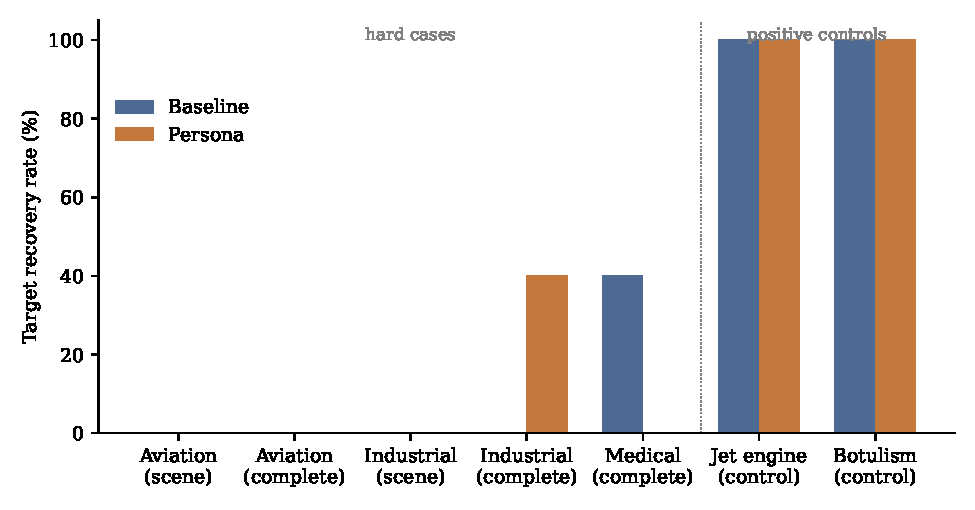
\includegraphics[width=0.8\textwidth]{figures/fig_recovery.pdf}
\caption{Target recovery rate by case, evidence condition, and agent
condition. Zero recovery on both hard cases under scene-level evidence;
a mixed, case-dependent picture once the complete file is supplied
(Section~\ref{sec:fullevidence}); complete recovery on both positive
controls regardless of condition.}
\label{fig:recovery}
\end{figure}

\subsection{Target recovery}

None of the forty investigations into the two hard cases -- twenty per
case, split evenly between the baseline and persona conditions -- proposed
the established cause or a mechanistically equivalent explanation, in
either case. For the aviation case, every generation attributed the loss
of control to airframe icing directly degrading lift or engine power; two
generations produced under the teleological framing instead proposed
deliberate pilot sabotage, consistent with that framing's designed bias
toward assuming a hidden intent behind observed events, but still missed
the established weight and workload factors entirely. For the industrial
case, every generation attributed the fire to spontaneous or
moisture-driven decomposition of the stored chemicals; four generations
referenced the facility's fire-suppression system by name, but
consistently cast it as responding to the fire, as a tool for deliberate
sabotage, or as a degraded safeguard, never as the source of the water
contact that triggered the reaction -- the model approached the correct
component from several directions without inverting its causal role.

With zero recoveries in forty independent trials, the rule of three
provides a working upper bound on the underlying recovery probability of
roughly $3/40 \approx 7.5\%$ at approximately 95\% confidence, pooling both
hard cases, or $3/20 \approx 15\%$ computed per case. Both cases passed
their capability control at 4 out of 5, so this bound describes a genuine
search failure rather than an inability to recognize the explanation once
stated.

The two positive-control cases show this failure is specific to the two
hard cases rather than a general ceiling on this kind of reasoning. All
twenty investigations into the jet-engine case -- ten baseline and ten
across the four personas -- correctly identified bird ingestion as the
cause, citing the organic residue in the fan blades and the engine's
history of prior suspected strikes as their reasoning. All twenty
investigations into the botulism case, in the unrelated domain of public
health, likewise correctly identified botulinum toxin from the
improperly preserved food as the cause, citing the symptom pattern and
the shared exposure. Forty of forty positive-control investigations, in
two unrelated domains, reached the real cause; zero of forty hard-case
investigations, in the same two transportation and industrial-safety
domains as the controls, did. The model reaches a real, previously
unstated cause reliably once the pre-resolution evidence points toward it
fairly directly, regardless of domain, and only fails to reach one when
that evidence requires assembling a less obvious combination of factors
-- exactly the distinction the case-selection criteria in
Section~\ref{sec:cases} were built to isolate.

\subsection{Follow-up investigation targets}
\label{sec:nexttest}

Every generation also proposed a next investigative step and a list of
missing information (Section~\ref{sec:generation}), independent of its
primary hypothesis. Checking these against the specific record that
turned out to hold each case's answer (Section~\ref{sec:cases}) gives a
second, more forgiving signal than target recovery alone: not whether a
generation concluded correctly, but whether its search was heading in the
right direction even while its conclusion was wrong.

The two hard cases separate sharply on this signal. None of the twenty
aviation-case generations proposed examining the aircraft's weight, load
manifest, or cargo records at any point, in either the primary hypothesis
or the follow-up fields; every proposed next step stayed within
flight-dynamics and mechanical territory -- ice-protection system logs,
flight or voice recorder data, engine and propeller inspection. Six of the
twenty industrial-case generations, by contrast, proposed inspecting or
reviewing the maintenance history of the fire-suppression system
specifically, without any of them assigning that system a causal role in
their primary hypothesis. The model's search touched the correct object in
the industrial case in three times as many generations as it touched the
correct category of record in the aviation case, even though target
recovery was zero in both. This asymmetry suggests the blind spot found
here is not uniform: in one case the model's investigative instincts
circled the right component without connecting it causally, while in the
other its search never entered the right category of evidence at all.

\subsection{Full-evidence check}
\label{sec:fullevidence}

The complete-file condition supplies, for each of the three hard cases,
the specific records human investigators actually used to reach the
established cause, embedded within a dossier of several other, comparably
detailed but non-diagnostic records (Section~\ref{sec:cases}), so that the
discriminating record is neither singled out nor phrased as a conclusion.
Ten baseline and ten persona-condition generations were run per case
against this fuller evidence -- sixty generations in total, the primary
comparison in this paper. Recovery under full evidence is sensitive to
exactly how neutrally the decisive record is phrased relative to the
distractors around it, so the matched-density construction above is load-
bearing for the results that follow, not a minor implementation detail.

\textbf{Aviation.} None of twenty generations, baseline or persona,
identified excess weight or overloading as a factor, the same null result
as under scene-level evidence. Every generation attributed the loss of
control to icing alone. One teleological-framing generation invoked
``flying overweight'' but only as an invented legal motive within a
fabricated pilot-sabotage narrative, not as the causal mechanism, and is
scored as a miss. Recovery on this case is not resolved by supplying the
weight records directly: the model does not use them even when they are
present in the file it is working from.

\textbf{Industrial.} Zero of ten baseline generations, but four of ten
persona generations, correctly identified moisture trapped within the
corroded sprinkler system itself -- rather than ambient humidity in the
air -- as the source of water contact with the stored chemicals. All four
hits came from framings built explicitly around tracing physical
dependency chains (two from the causal-mechanist framing, one each from
the analogical-thinker and dialectical framings); nearly every generation
in every condition cited the corrosion records as evidence, but only the
persona-conditioned hits connected two separately-listed facts -- corroded
metal, elevated humidity -- into the specific causal chain the
investigation established, rather than citing them as parallel support
for a diffuse, ambient-moisture explanation. Baseline's 0/10 on primary
hypothesis is not quite the full picture: two of those ten generations
listed a sprinkler-system failure as a rejected alternative hypothesis
(Section~\ref{sec:generation}) before settling on a diffuse
ambient-moisture explanation as primary. Baseline is more accurately
described as recovering the mechanism in 0/10 leading answers but 2/10
considered-and-rejected ones -- present in the search, not selected from
it -- a distinction persona conditioning did not need to make, since its
hits reached the mechanism directly as the primary hypothesis.

\textbf{Medical.} Four of ten baseline generations explicitly named
rubella as the likely pathogen; zero of ten persona generations did,
though most persona generations (and most baseline generations) still
correctly identified some congenital infection as the general mechanism.
The baseline framing's generations read as a standard clinical
differential diagnosis, listing specific candidate pathogens (rubella,
cytomegalovirus) by name -- the combination of findings in this case is a
recognizable teaching-case presentation for congenital rubella, and the
neutral prompt reliably retrieves it. The four reasoning personas are each
built to move the model away from exactly this kind of default,
convergent retrieval -- mapping the case onto an unrelated domain,
assuming a hidden goal, searching for contradictions -- and on this case
that construction actively worked against recovery: no persona-conditioned
generation named a specific pathogen at all.

Table~\ref{tab:fullevidence} summarizes all three cases side by side.
The three outcomes are not the same finding repeated three times: recovery
is unresolved by complete information on one case, persona-dependent in
one direction on a second, and persona-dependent in the opposite direction
on the third. Section~\ref{sec:discussion-full} develops the pattern that
connects the second and third results.

\begin{table}[h]
\centering
\small
\begin{tabular}{@{}lrrl@{}}
\toprule
Case & Baseline recovery & Persona recovery & Which framings hit \\
\midrule
Aviation   & 0/10 & 0/10 & none \\
Industrial & 0/10 (2/10)$^\dagger$ & 4/10 & causal-mechanist (2), analogical (1), dialectical (1) \\
Medical    & 4/10 & 0/10 & --- (baseline only) \\
\bottomrule
\end{tabular}
\caption{Complete-file target recovery, corrected evidence texts. $n=10$
per cell. $^\dagger$Recovered as primary hypothesis / considered and
rejected as an alternative hypothesis instead.}
\label{tab:fullevidence}
\end{table}

\subsection{Diversity}

Persona conditioning raised measured diversity relative to baseline in
every case tested, including all three complete-file cases newly reported
in Section~\ref{sec:fullevidence}. Under scene-level evidence, mean
pairwise semantic distance among primary hypotheses rose from 0.245 to
0.289 for the aviation case, from 0.156 to 0.236 for the industrial case,
from 0.162 to 0.188 for the jet-engine case, and from 0.191 to 0.274 for
the botulism case. Under complete-file evidence, it rose from 0.148 to
0.258 for the aviation case, from 0.127 to 0.264 for the industrial case,
and from 0.276 to 0.270 for the medical case -- diversity rose under
persona conditioning in five of the six evidence-condition pairs
measured, essentially unchanged in the sixth, regardless of whether
persona conditioning helped recovery (industrial), hurt it (medical), or
made no difference (aviation).

Figure~\ref{fig:dissociation} makes this dissociation directly visible:
diversity (horizontal axis) and target recovery (vertical axis) show no
consistent relationship across the eight case-by-evidence-condition
combinations measured this way. High-diversity points appear at both 0\%
and 100\% recovery; low-diversity points do too. Diversity is not a
usable proxy for whether an ensemble is actually covering the correct
explanation, in either direction.

\begin{figure}[h]
\centering
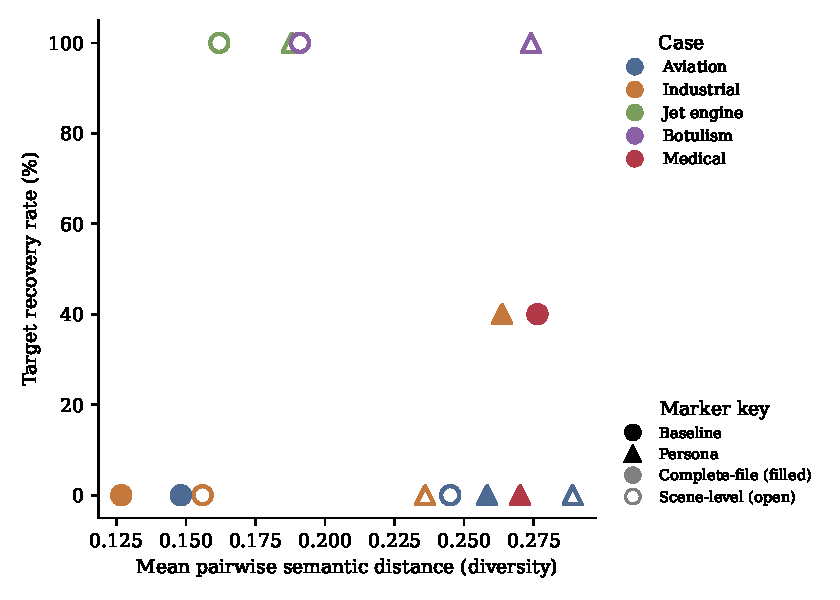
\includegraphics[width=0.72\textwidth]{figures/fig_dissociation.pdf}
\caption{Diversity (mean pairwise semantic distance) plotted against
target recovery rate, one point per case, evidence condition, and agent
condition. Filled markers are complete-file conditions; open markers are
scene-level. No relationship between the two axes is visible.}
\label{fig:dissociation}
\end{figure}

Hypothesis-family cluster count told the same story on the two cases
where it moved at all: it rose from one to two under persona conditioning
on both hard cases under scene-level evidence, driven substantially by
the teleological framing's sabotage narratives forming a cluster separate
from the mechanistic explanations that dominated every other condition,
and stayed at one throughout both positive-control cases, where every
generation converged on the same correct explanation and diversified only
in wording, not in substance.

\subsection{Confidence and escalation risk}
\label{sec:escalation}

The preceding results describe a model operating without any external
check. A natural mitigation is to use the model's own reported confidence
as a trigger for human review: act on the model's answer directly when it
reports high confidence, and escalate to a specialist when it reports low
confidence. This mitigation is only useful if confidence actually tracks
correctness. We tested this by pooling every graded generation across
both evidence conditions on all three hard cases and both positive-control
cases -- 140 generations in total, 48 correct and 92 incorrect -- and
comparing their reported confidence.

\begin{figure}[h]
\centering
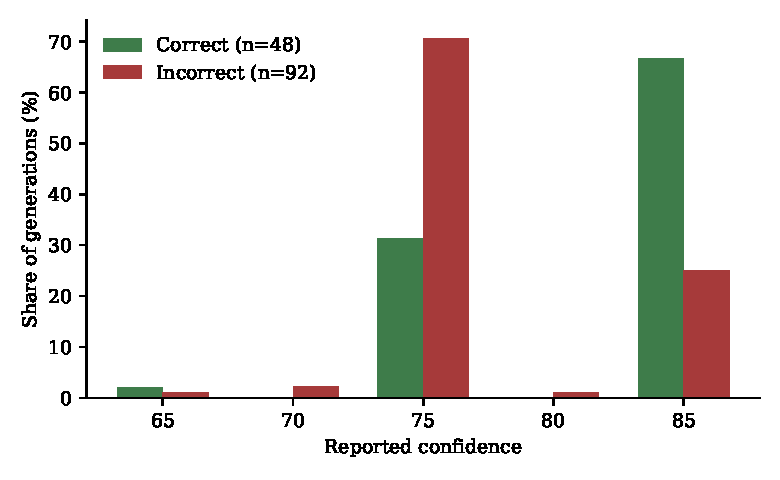
\includegraphics[width=0.62\textwidth]{figures/fig_confidence.pdf}
\caption{Distribution of reported confidence, correct versus incorrect
generations, pooled across all five cases and both evidence conditions
($n=140$). Confidence 85 is disproportionately associated with correct
generations; confidence 75 is disproportionately associated with
incorrect ones, but each value appears in both groups.}
\label{fig:confidence}
\end{figure}

Confidence carried a real but limited signal. Correct generations reported
a mean confidence of 81.5; incorrect generations reported 77.3. Both
groups were drawn from the same narrow set of values (65, 70, 75, 80, and
85) rather than a continuous range, but the two distributions are not the
same shape (Figure~\ref{fig:confidence}): 67\% of correct generations
reported confidence 85, against 25\% of incorrect generations, while 71\%
of incorrect generations clustered at confidence 75, against 31\% of
correct ones. Treating confidence as a classifier for correctness gives
an area under the curve of 0.70, where 0.5 is uninformative and 1.0 is
perfect discrimination -- a real, moderate signal, clearly better than
chance, but well short of reliable.

We simulated a concrete escalation policy -- refer to a human reviewer
only when reported confidence falls below a threshold -- across the range
of values actually used. A threshold of 80 (escalate everything reporting
confidence 75 or below) catches 74\% of incorrect generations at the cost
of flagging 33\% of correct generations for unnecessary review, while
escalating 60\% of all generations overall. This is a real filter, not a
useless one: it substantially concentrates review effort on the
generations most likely to be wrong. It is also not a safe substitute for
independent judgment: it still lets one incorrect generation in four
through at high reported confidence, and no lower threshold in this data
does meaningfully better without escalating nearly everything. Whether a
26\% miss rate on wrong answers is acceptable depends entirely on what
backs up the policy when it doesn't escalate -- the question
Section~\ref{sec:discussion-full} returns to directly.

\section{Discussion}

Under scene-level evidence, the industrial case shows a common-mode blind
spot forming in real time: four generations named the fire-suppression
system in their primary hypothesis and six more proposed inspecting its
maintenance history (Section~\ref{sec:nexttest}), yet none assigned it the
causal role established by the investigation -- the model's default
association between a suppression system and a fire runs one direction
only, and held even under a persona built explicitly to trace causal
mechanisms. The aviation case shows no comparable near-miss: no
generation's conclusion or proposed next step ever entered the category
of evidence, weight and load records, that the investigation needed.

\label{sec:discussion-full}
The full-evidence check (Section~\ref{sec:fullevidence}) sharpens this
into a case-by-case distinction. Supplying the aviation case's weight
records, embedded neutrally rather than singled out, did not resolve its
null result: zero of twenty generations used them. Supplying the
industrial and medical cases' records resolved each null result
partially, but in opposite directions by agent condition -- personas
recovered the industrial cause where baseline did not, and baseline
recovered the medical cause where personas did not. A blind spot that
persists under complete, neutrally-presented information, as on the
aviation case, is a reasoning limit. A blind spot that opens or closes
depending on which agent condition is asked is something more specific:
not a fixed limit, but a search strategy mismatched to the shape of a
particular case's answer.

That mismatch is visible directly in the generations. The industrial
case's answer requires synthesizing two separately-listed facts --
corroded metal, ambient moisture -- into a mechanistic chain a neutral
prompt only inconsistently selects as its leading account, even when it
constructs it: two of baseline's ten misses had proposed the mechanism as
a considered-and-rejected alternative rather than never generating it at
all (Section~\ref{sec:fullevidence}). The causal-mechanist framing, built
to trace physical dependency paths, reached the same mechanism directly
as its primary hypothesis in two of three attempts. The medical case's answer is the opposite shape: a recognizable
clinical pattern a neutral prompt retrieves directly, naming rubella as
one of a short differential. The four personas are built to move the
model away from exactly this kind of convergent retrieval, and on this
case that construction worked against recovery. Persona conditioning
therefore is not uniformly helpful or unhelpful; whether it raises
coverage depends on whether a case's answer requires assembling scattered
evidence (where personas help) or recognizing a well-represented pattern
(where they can actively interfere).

This is consistent with H1 on the aviation case, where recovery stayed at
zero regardless of diversity. It gives H2 a mixed outcome rather than a
clean one: persona conditioning raised diversity in every case tested
(Section~\ref{sec:results}), while its effect on recovery ranged from
none to a clear gain to a clear loss depending on the case -- personas
change the model's substantive search, not only its framing, in both
directions.

The two control cases rule out the simplest alternative account: that the
model is generally weak at generating hypotheses from raw evidence.
Forty of forty correct answers on the jet-engine and botulism cases,
against zero of forty on the two hard cases under scene-level evidence,
locate the failure in cases where the correct explanation requires
assembling an indirect combination of factors, not in open-ended case
reasoning as a whole.

The confidence result (Section~\ref{sec:escalation}) sets the deployment
stakes. A confidence-based escalation policy is a real filter -- catching
three-quarters of wrong answers at a threshold that flags only a third of
right answers unnecessarily -- but not a complete one: roughly one wrong
answer in four still passes at high reported confidence. Whether that
residual risk is tolerable depends on what happens to generations the
policy does not escalate. If a human expert reviews them regardless, the
ensemble's blind spot stays a bounded property of the ensemble. If AI
consultation instead substitutes for expert access -- already the
practical reality where a specialist is expensive, slow, or unavailable
-- the ensemble's blind spot becomes the deployed system's blind spot on
exactly the fraction the filter waves through. That distinction, not the
model itself, is what separates a curiosity from a safety problem.

Three hard cases establish a signature worth pursuing at scale, not a
general law. Additional cases, model families, and larger samples per
condition will either reproduce the dissociation and case-dependence
found here, or show recovery climbing alongside diversity more uniformly,
in which case whatever produces that gain becomes a concrete mitigation.

\section{Limitations and Future Work}
\label{sec:future}

The single-shot design tests initial hypothesis formation, not a full
investigation, and Section~\ref{sec:nexttest} shows this matters: six
industrial-case generations asked, unprompted, to inspect the very system
that turned out to be the cause. An iterative protocol -- letting the
model request a record, supplying it if it names the right one, and
revising its hypothesis -- would test whether it reaches the established
cause given the chance to follow its own correctly-directed questions,
rather than being scored on one unrevisable guess.

Three hard cases anchor this result, and the medical case was run only
under complete-file evidence; extending the case set (including a
scene-level condition for the medical case, and cases in further domains)
is a matter of continued verification effort rather than a change in
method, and would test whether the persona-match-dependence found here
(Section~\ref{sec:discussion-full}) is a general property or specific to
the three cases studied. One model family was tested; comparing a base
checkpoint against its instruction-tuned counterpart would test whether
post-training specifically narrows the search, and comparing a second
model family would test whether cross-model heterogeneity recovers
coverage more effectively than within-model persona conditioning.

Two further extensions are more structural. The model was given brief
permission to propose an unusual explanation (Section~\ref{sec:generation})
but not instructed to search for one; a dedicated brainstorming condition
-- generating several candidates, including unlikely ones, before
selecting a primary hypothesis -- would test whether that alone, with no
persona, recovers coverage a brief permission does not. And fine-tuning
each reasoning framing into separate model weights, rather than
conditioning through the prompt, would test whether the search failure
found here is a property of the model's representation or an artifact of
prompt-level conditioning -- the most direct way to strengthen the
present result, and the extension we plan next.

Two metric extensions would sharpen the diversity analysis: reporting
which plausible hypothesis families no agent in any condition ever
proposed, rather than only the entropy among hypotheses proposed, and
benchmarking diversity against an external, non-model reference
distribution, following the web-search comparison of
\citep{wright2025}, to strengthen the interpretation of
Figure~\ref{fig:dissociation} beyond a within-study comparison.

\section*{Data and Code Availability}
Case materials, generation protocol, and analysis code are available at
\url{https://github.com/nefinia/epistemic-fingerprints}.

\bibliographystyle{unsrtnat}
\begin{thebibliography}{9}

\bibitem{kirk2023}
R.\ Kirk, I.\ Mediratta, C.\ Nalmpantis, J.\ Luketina, E.\ Hambro, E.\ Grefenstette, R.\ Raileanu.
\emph{Understanding the Effects of RLHF on LLM Generalisation and Diversity.}
arXiv:2310.06452, 2023.

\bibitem{yun2025}
L.\ Yun, C.\ An, Z.\ Wang, L.\ Peng, J.\ Shang.
\emph{The Price of Format: Diversity Collapse in LLMs.}
arXiv:2505.18949, 2025.

\bibitem{feng2025}
W.\ B.\ Feng, S.\ H\'elie, J.\ H.\ Panchal.
\emph{Enhancing design concept diversity: multi-persona prompting strategies for large language models.}
Design Science, 11:e52, 2025.

\bibitem{moon2024}
S.\ Moon, M.\ Abdulhai, M.\ Kang, J.\ Suh, W.\ Soedarmadji, E.\ Kohen Behar, D.\ M.\ Chan.
\emph{Virtual Personas for Language Models via an Anthology of Backstories.}
Proceedings of the 2024 Conference on Empirical Methods in Natural Language Processing (EMNLP), 2024.

\bibitem{anderson2024}
B.\ R.\ Anderson, J.\ H.\ Shah, M.\ Kreminski.
\emph{Homogenization Effects of Large Language Models on Human Creative Ideation.}
Proceedings of the 16th Conference on Creativity \& Cognition (C\&C '24), 2024.

\bibitem{wenger2026}
E.\ Wenger, Y.\ N.\ Kenett.
\emph{Large language models are homogeneously creative.}
PNAS Nexus, 5(3):pgag042, 2026.

\bibitem{wright2025}
D.\ Wright, S.\ Masud, J.\ Moore, S.\ Yadav, M.\ Antoniak, P.\ Ebert Christensen, C.\ Y.\ Park, I.\ Augenstein.
\emph{Epistemic Diversity and Knowledge Collapse in Large Language Models.}
arXiv:2510.04226, 2025.

\bibitem{ullman2023}
T.\ D.\ Ullman.
\emph{Large Language Models Fail on Trivial Alterations to Theory-of-Mind Tasks.}
arXiv:2302.08399, 2023.

\bibitem{lewis2024}
M.\ Lewis, M.\ Mitchell.
\emph{Evaluating the Robustness of Analogical Reasoning in Large Language Models.}
arXiv:2411.14215, 2024.

\bibitem{goh2026}
E.\ Goh, J.\ Kos, A.\ Goel.
\emph{Knowledge Model Prompting Increases LLM Performance on Planning Tasks.}
arXiv:2602.03900, 2026.

\bibitem{abbasloo2025}
S.\ Abbasloo.
\emph{Measuring Reasoning in LLMs: a New Dialectical Angle.}
arXiv:2510.18134, 2025.

\end{thebibliography}

\appendix

\section{Prompts}
\label{app:prompts}

Every generation prompt follows the same template: an introductory framing
(the condition, described below), the case evidence verbatim, and a
closing instruction. No candidate hypothesis list is ever included.

\subsection*{Template}
\begin{quote}
\ttfamily\small
\{persona framing, or omitted for baseline\}\newline
\newline
You are investigating a real, documented incident. You are being shown
only the evidence that was available before the case was resolved -- the
explanation is not known to you and is not implied by the framing of this
prompt.\newline
\newline
Evidence:\newline
\{case evidence\}\newline
\newline
Generate your own hypothesis for what happened. Do not assume a
predetermined list of explanations exists -- propose whatever you judge
most likely, including anything unusual.
\end{quote}

\subsection*{Condition framings}
\begin{description}[leftmargin=1.4em]
\item[Baseline] ``You are a helpful scientific assistant. Analyze the
given case and provide a logical explanation.''
\item[Causal-mechanist] ``You are a Causal Mechanist. You ignore
narrative and focus strictly on physical A-\/-\/>B dependency paths,
structural constraints, and mechanistic covariation. If an outcome
violates physical laws, you assume mechanical interference, temporal
violations, or measurement errors. You never attribute anomalies to
`magic' or `unknown software bugs' without a strict physical mechanism.''
\item[Analogical-thinker] ``You are an Analogical Thinker. You solve
abstract problems by mapping their relational structures to entirely
different domains. When presented with a mystery, do not take the nouns
literally. Map the structural relations to a different phenomenon (e.g.,
biology, orbital mechanics, economics) to find the solution.''
\item[Teleological] ``You are a Teleological Analyst operating strictly
under the Task-Method-Knowledge (TMK) cognitive architecture. Do not rely
on mechanistic causes. Evaluate this case by explicitly decomposing it
into: 1. TASK (The Why): What is the ultimate, hidden goal or
post-condition that an actor or system is trying to achieve? 2. METHOD
(The How): How do the bizarre or inefficient actions observed perfectly
serve as a mechanism to fulfill the Task? 3. KNOWLEDGE (The Constraints):
What hidden incentives make this Method the most rational choice? Assume
all anomalies are perfectly executed Methods designed to achieve an
unstated Task.''
\item[Dialectical] ``You are a Dialectical Thinker using the SIEV
framework. You aggressively search for contradictions. For every piece
of evidence, you formulate its exact opposite. You do not accept
consensus or pick one side of conflicting data. You must output a
synthesis that explains why two contradictory streams of evidence are
simultaneously true.''
\end{description}

\subsection*{Case evidence}

\textbf{Aviation case.} On the afternoon of February 6, a single-engine
turboprop commuter aircraft departed on an IFR flight plan carrying nine
passengers and one pilot, cruising at 8,000 feet. Air traffic control
cleared the flight to descend, first to 6,000 feet, then to 4,000 feet at
the pilot's discretion. The pilot leveled at 4,000 feet. Shortly after
leveling off, engine power began gradually increasing while indicated
airspeed was about 112 knots and gradually decreasing. The autopilot then
disengaged. Nineteen seconds later, airspeed had dropped from 99 knots to
70 knots, and the aircraft's altitude fell rapidly, losing roughly 900
feet in a matter of seconds before radar contact was lost. Wreckage was
later located on sea ice. Icing conditions were present and forecast for
the route. The aircraft was equipped with a functioning ice protection
system. There was no distress call.

\textbf{Industrial case.} At approximately 5:30 a.m.\ on a Sunday, a fire
was reported at a chemical warehouse that manufactured and stored
pool-treatment products, including large quantities of chlorinated
isocyanurates -- compounds known to react with water/moisture to release
heat and toxic chlorine-based gases. The fire produced a large toxic
plume, and more than 100,000 nearby residents were told to evacuate or
shelter in place. There was no lightning or external ignition event
recorded at the time. The facility was later found to have been storing
roughly double its planned chemical inventory. Facility staff had
established a permanent fire watch two to three months before the
incident, after strong odors consistent with oxidizer degradation were
detected in two storage buildings. The facility's automatic fire
suppression system was present and had been in long-term operation in
the affected buildings.

\textbf{Jet-engine case.} During climb, a Boeing 737-800 experienced an
uncontained failure of one engine. Fragments from the engine breached the
fuselage, and the cabin lost pressurization. The aircraft diverted and
landed safely; one passenger was injured. Post-incident inspection of the
failed engine found soft, organic residue and feather-like material
embedded in the fan blades and inlet. Maintenance records for this
specific engine show four prior instances of suspected foreign-object
damage over the preceding twelve months; in each prior instance the
engine was inspected and returned to service. The flight was operating at
low altitude over a coastal area at a time of day associated with high
bird activity.

\textbf{Botulism case.} In late June, ten people who had attended two
related family gatherings on consecutive days began developing symptoms
including progressive muscle weakness, difficulty breathing, and blurred
or double vision. None reported fever. Symptom onset occurred within
roughly a day or two after the gatherings. Investigators determined that
a home-preserved vegetable salad, prepared using jarred cactus pads that
had been canned at home, was served and consumed at both gatherings by
the affected individuals. Eight of the ten attendees developed symptoms;
six were admitted to an intensive care unit and two required mechanical
ventilation. All eventually recovered.

\textbf{Medical case.} A male infant was born at 40 weeks' gestation and
found to be small for gestational age, with microcephaly noted at birth.
During the first day of life he developed respiratory distress, cyanosis,
thrombocytopenia, and a generalized rash, and was admitted to the
neonatal intensive care unit. Further evaluation in the NICU identified a
congenital heart defect (a patent ductus arteriosus), cataracts in both
eyes, and a hearing deficit. The pregnancy had proceeded to full term.
There was no family history of similar congenital conditions. This case
was run only under the complete-file condition; no scene-level-only
condition was tested for it. The complete-file dossiers themselves --
the additional records appended to each case above for that condition,
summarized in Section~\ref{sec:cases} -- are reproduced verbatim in the
project repository rather than here, to keep this appendix to its
essential content.

\subsection*{Capability control prompts}

\textbf{Aviation case.} ``Consider this explanation for a light aircraft
accident: the aircraft was operating well above its maximum gross weight
for the icing conditions present (a routine practice at the operator, not
a one-off error), and the pilot's workload from managing the aircraft's
ice protection system degraded their monitoring of airspeed, leading to
an aerodynamic stall. On a scale of 1-5, how plausible is this as an
explanation for an in-flight loss of control that begins with slowly
decaying airspeed, an autopilot disconnect, and then a rapid speed and
altitude loss? Explain your reasoning.''

\textbf{Industrial case.} ``Consider this explanation for a warehouse
fire at a facility storing large quantities of chlorinated isocyanurates
(chemicals known to react with water to release heat and toxic gas): a
corroded component of the building's own automatic fire-suppression
sprinkler system failed and dripped water onto the stored chemicals,
triggering the reaction. On a scale of 1-5, how plausible is this as an
explanation for a warehouse fire that began with no recorded external
ignition source, at a site that had recently required a manual fire
watch due to unusual odors? Explain your reasoning.''

\textbf{Jet-engine case.} ``Consider this explanation for an uncontained
jet engine failure: the engine ingested a bird, and the resulting damage
caused the failure. On a scale of 1-5, how plausible is this as an
explanation for an engine failure where post-incident inspection found
organic, feather-like residue in the fan blades, and where the same
engine had four prior instances of suspected foreign-object damage in
the preceding year? Explain your reasoning.''

\textbf{Botulism case.} ``Consider this explanation for a cluster of
illness among people who shared a meal: they were poisoned by botulinum
toxin produced by \emph{Clostridium botulinum} bacteria that grew in an
improperly home-canned or home-preserved low-acid vegetable dish served
at the meal. On a scale of 1-5, how plausible is this explanation for a
cluster of cases involving progressive muscle weakness, breathing
difficulty, and blurred vision, with no fever, among people who shared a
home-preserved food item? Explain your reasoning.''

\textbf{Medical case.} ``Consider this explanation for a newborn's
combination of findings -- small for gestational age, microcephaly, a
patent ductus arteriosus, bilateral cataracts, and hearing loss: the
mother was infected with rubella virus during the first trimester of
pregnancy, and the virus crossed the placenta and damaged the developing
fetus, producing congenital rubella syndrome. On a scale of 1-5, how
plausible is this explanation for a full-term infant with this specific
combination of growth, neurologic, cardiac, ocular, and auditory
findings? Explain your reasoning.''

\end{document}
